%% Basierend auf einer TeXnicCenter-Vorlage von Mark Müller
%%%%%%%%%%%%%%%%%%%%%%%%%%%%%%%%%%%%%%%%%%%%%%%%%%%%%%%%%%%%%%%%%%%%%%%

% Wählen Sie die Optionen aus, indem Sie % vor der Option entfernen  
% Dokumentation des KOMA-Script-Packets: scrguide

%%%%%%%%%%%%%%%%%%%%%%%%%%%%%%%%%%%%%%%%%%%%%%%%%%%%%%%%%%%%%%%%%%%%%%%
%% Optionen zum Layout des Artikels                                  %%
%%%%%%%%%%%%%%%%%%%%%%%%%%%%%%%%%%%%%%%%%%%%%%%%%%%%%%%%%%%%%%%%%%%%%%%
\documentclass[%
%a5paper,							% alle weiteren Papierformat einstellbar
%landscape,						% Querformat
%10pt,								% Schriftgröße (12pt, 11pt (Standard))
%BCOR1cm,							% Bindekorrektur, bspw. 1 cm
%DIVcalc,							% führt die Satzspiegelberechnung neu aus
%											  s. scrguide 2.4
%twoside,							% Doppelseiten
%twocolumn,						% zweispaltiger Satz
%halfparskip*,				% Absatzformatierung s. scrguide 3.1
%headsepline,					% Trennline zum Seitenkopf	
%footsepline,					% Trennline zum Seitenfuß
%titlepage,						% Titelei auf eigener Seite
%normalheadings,			% Überschriften etwas kleiner (smallheadings)
%idxtotoc,						% Index im Inhaltsverzeichnis
%liststotoc,					% Abb.- und Tab.verzeichnis im Inhalt
%bibtotoc,						% Literaturverzeichnis im Inhalt
%abstracton,					% Überschrift über der Zusammenfassung an	
%leqno,   						% Nummerierung von Gleichungen links
%fleqn,								% Ausgabe von Gleichungen linksbündig
%draft								% überlangen Zeilen in Ausgabe gekennzeichnet
]
{scrartcl}

%\pagestyle{empty}		% keine Kopf und Fußzeile (k. Seitenzahl)
%\pagestyle{headings}	% lebender Kolumnentitel

%% Deutsche Anpassungen %%%%%%%%%%%%%%%%%%%%%%%%%%%%%%%%%%%%%
\usepackage[english]{babel}
\usepackage[T1]{fontenc}
\usepackage[utf8]{inputenc}

\usepackage{amsthm} % Theorem-Packet
\usepackage{amsmath}
\usepackage{amssymb}

\usepackage{stmaryrd} % Blitzsymbol
\usepackage{fancyhdr} % Für Kopfzeile
\usepackage{graphicx} % Einbinden von Grafiken
\usepackage{bbding} % Für das Häckchen
\usepackage{amscd} % Kommutative Diagramme
\usepackage{mathtools} % Für das Definitionssymbol

\usepackage{listings}
\usepackage{courier}

\pagestyle{fancy}
\lhead{Computational Science I}\chead{Exercise notes: Combinatorics}\rhead{HS 2013} % Kopfzeile

\newtheoremstyle{plain}%  name
  {.5\baselineskip}% Space above
  {.5\baselineskip}% Space below
  {}% Body font
  {}% Indent amount (empty = no indent, \parindent = para indent)
  {\bfseries}% Thm head font
  {:}% Punctuation after thm head
  { }% Space after thm head: " " = normal interword space; \newline = linebreak
  {}% Thm head spec (can be left empty, meaning `normal')
  
\makeatletter % Matrizen mit opitonalen Linien
\renewcommand*\env@matrix[1][*\c@MaxMatrixCols c]{%
  \hskip -\arraycolsep
  \let\@ifnextchar\new@ifnextchar
  \array{#1}}
\makeatother

\theoremstyle{plain}
\newtheorem*{bsp}{Beispiel} % Beispiele ohne Nummerierung
\newtheorem*{bws}{Beweis} % Beweise ohne Nummerierung 
\newenvironment{beweis}{\begin{bws}~\vspace{0.5\baselineskip}}{\hfill $\qedsymbol$\end{bws}}
\newenvironment{beispiel}{\begin{bsp}~\vspace{0.5\baselineskip}}{\end{bsp}}

\usepackage{lmodern} % Type1-Schriftart für nicht-englische Texte

\usepackage{enumerate}

\renewcommand\theenumi{\roman{enumi}}
\renewcommand\labelenumi{\theenumi)}

%% Packages für Grafiken & Abbildungen %%%%%%%%%%%%%%%%%%%%%%
%\usepackage{graphicx} %%Zum Laden von Grafiken
%\usepackage{subfig} %%Teilabbildungen in einer Abbildung
%\usepackage{tikz} %%Vektorgrafiken aus LaTeX heraus erstellen

%\setlength{\parindent}{0pt} % kein Einzug


%% Beachten Sie:
%% Die Einbindung einer Grafik erfolgt mit \includegraphics{Dateiname}
%% bzw. über den Dialog im Einfügen-Menü.
%% 
%% Im Modus "LaTeX => PDF" können Sie u.a. folgende Grafikformate verwenden:
%%   .jpg  .png  .pdf  .mps
%% 
%% In den Modi "LaTeX => DVI", "LaTeX => PS" und "LaTeX => PS => PDF"
%% können Sie u.a. folgende Grafikformate verwenden:
%%   .eps  .ps  .bmp  .pict  .pntg


%% Bibliographiestil %%%%%%%%%%%%%%%%%%%%%%%%%%%%%%%%%%%%%%%%%%%%%%%%%%
%\usepackage{natbib}

\begin{document}

\lstset{basicstyle=\ttfamily, breakatwhitespace=false, breaklines=true, frame=single, xleftmargin=\parindent, aboveskip=\baselineskip, belowskip=\baselineskip}

%\pagestyle{empty} %%Keine Kopf-/Fusszeilen auf den ersten Seiten.


%%%%%%%%%%%%%%%%%%%%%%%%%%%%%%%%%%%%%%%%%%%%%%%%%%%%%%%%%%%%%%%%%%%%%%%
%% Ihr Artikel                                                       %%
%%%%%%%%%%%%%%%%%%%%%%%%%%%%%%%%%%%%%%%%%%%%%%%%%%%%%%%%%%%%%%%%%%%%%%%

%% eigene Titelseitengestaltung %%%%%%%%%%%%%%%%%%%%%%%%%%%%%%%%%%%%%%%    
%\begin{titlepage}
%Einsetzen der TXC Vorlage "Deckblatt" möglich
%\end{titlepage}

%% Angaben zur Standardformatierung des Titels %%%%%%%%%%%%%%%%%%%%%%%%
\titlehead{\center{University of Zurich - HS 2013}}
%\subject{Typisierung}
\title{Computational Science I\\Exercise notes: Combinatorics\\\rule{1.0\textwidth}{1.0pt}}
\author{Tobias Grubenmann}
%\and{Der Name des Co-Autoren}
%\thanks{Fußnote}			% entspr. \footnote im Fließtext
%\date{}							% falls anderes, als das aktuelle gewünscht
%\publishers{Herausgeber}

%% Widmungsseite %%%%%%%%%%%%%%%%%%%%%%%%%%%%%%%%%%%%%%%%%%%%%%%%%%%%%%
%\dedication{Widmung}

\maketitle 						% Titelei wird erzeugt

%% Zusammenfassung nach Titel, vor Inhaltsverzeichnis %%%%%%%%%%%%%%%%%
%\begin{abstract}
% Für eine kurze Zusammenfassung des folgenden Artikels.
% Für die Überschrift s. \documentclass[abstracton].
%\end{abstract}

%% Erzeugung von Verzeichnissen %%%%%%%%%%%%%%%%%%%%%%%%%%%%%%%%%%%%%%%
%\tableofcontents			% Inhaltsverzeichnis
%\listoftables				% Tabellenverzeichnis
%\listoffigures				% Abbildungsverzeichnis


%% Der Text %%%%%%%%%%%%%%%%%%%%%%%%%%%%%%%%%%%%%%%%%%%%%%%%%%%%%%%%%%%

\section*{Exercise 1}

To find all independent solution for the eight-queen problem I first searched for all dependent solution using an integer representation for convenience. After that I converted the solutions to a complex representation, again for convenience. Now, I pick up a solution and delete all rotated and/or reflected solutions. The remaining solutions are all independent solutions of the eight-queen problem.

The function \texttt{getIndependentSolutions} returns the independent solutions of the eight-queen problem:

\lstinputlisting[language=Python]{../EightQueens.py}

From the function \texttt{getIndependentSolutions} we will get the following \textbf{12} independent solutions:

\lstinputlisting{../EightQueensSolutions.txt}

\section*{Exercise 2}

First, I generate all the 64 different codons with \texttt{generateCodons}. The codons are encoded by a triple of numbers where $A=0$, $C=1$, $G=2$, $T=3$.We can then just convert the codons into diamonds by the formula:

\begin{equation*}
diamond = (codon_{1}, codon_{2}, 3-codon_{3}, 3-codon_{2})
\end{equation*}

Like in the eight-queens problem, I can now select a diamond and delete all diamonds which are reserved or start at the other corner.

\lstinputlisting[language=Python]{../GamowDiamonds.py}

The function \texttt{getDifferentGamowDiamonds} returns all 20 different Gamow-diamonds:

\lstinputlisting{../GamowDiamonds.txt}

\section*{Exercise 3}

I used the \textbf{ELANE} gene to make a comparison between humans, chimpanzees, dogs and cats. First, I downloaded the sequences corresponding to the species using the following code:

\lstinputlisting[language=Python]{../SequenceDownload.py}

Afterward, I made an sequence alignment analysis by putting the downloaded sequence in another code. The following code plots a dot whenever five consecutive characters matches in two different sequences. The coordinates of the plot indicates the position of the five characters in the first and second sequence. In addition, a number indicating how many matches where found for a given pair of sequences is also printed:

\lstinputlisting[language=Python]{../SequenceAlignment.py}

The figures below shows the alignment plot for the ELANE gene for the different species:

\begin{center}
\centering
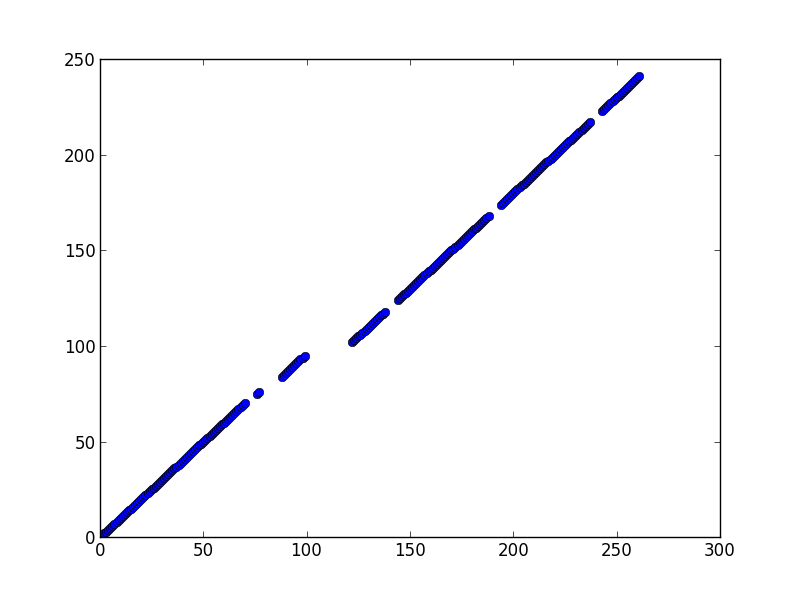
\includegraphics[width=0.6\linewidth]{../HumanChimpanzeeAlignment.png}
\captionof{figure}{Human - chimpanzee alignment for the ELANE gene. 5 character region match.}
\end{center}

\begin{center}
\centering
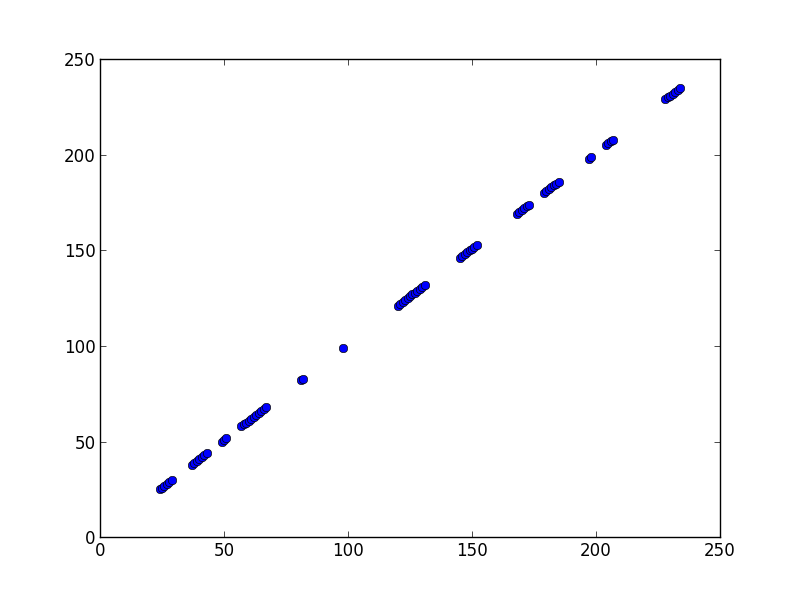
\includegraphics[width=0.6\linewidth]{../HumanDogAlignment.png}
\captionof{figure}{Human - dog alignment for the ELANE gene. 5 character region match.}
\end{center}

\begin{center}
\centering
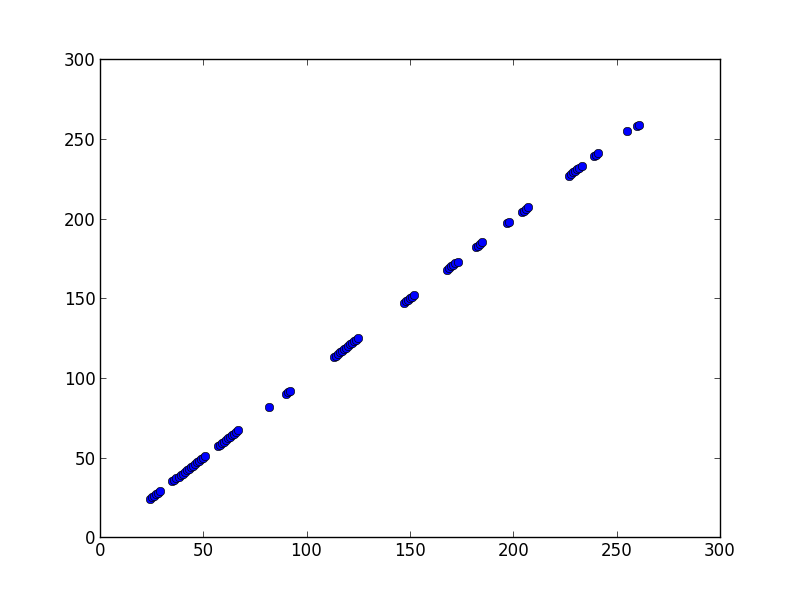
\includegraphics[width=0.6\linewidth]{../HumanCatAlignment.png}
\captionof{figure}{Human - cat alignment for the ELANE gene. 5 character region match.}
\end{center}

\begin{center}
\centering
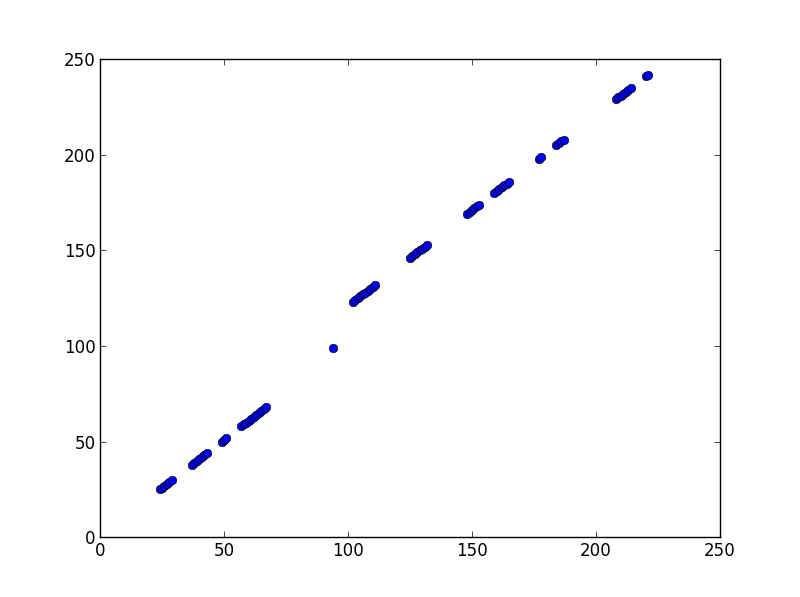
\includegraphics[width=0.6\linewidth]{../ChimpanzeeDogAlignment.png}
\captionof{figure}{Chimpanzee - dog alignment for the ELANE gene. 5 character region match.}
\end{center}

\begin{center}
\centering
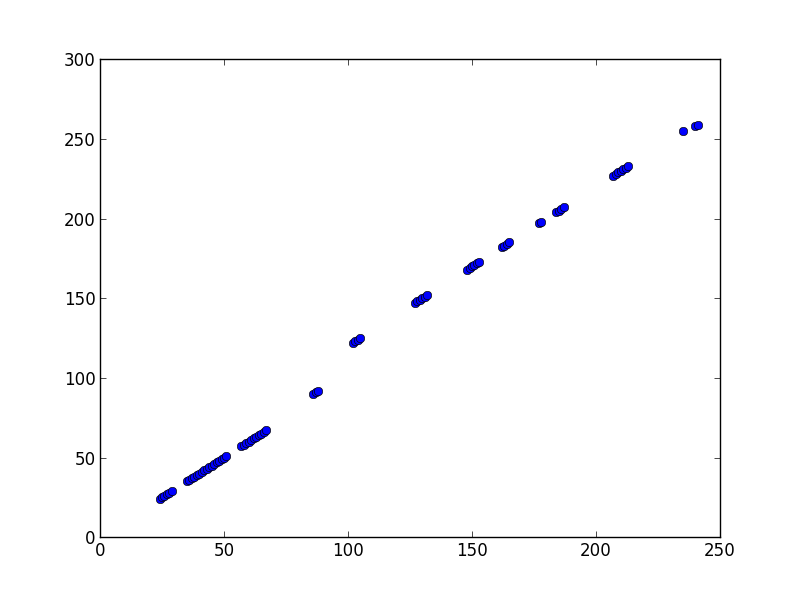
\includegraphics[width=0.6\linewidth]{../ChimpanzeeCatAlignment.png}
\captionof{figure}{Chimpanzee - cat alignment for the ELANE gene. 5 character region match.}
\end{center}

\begin{center}
\centering
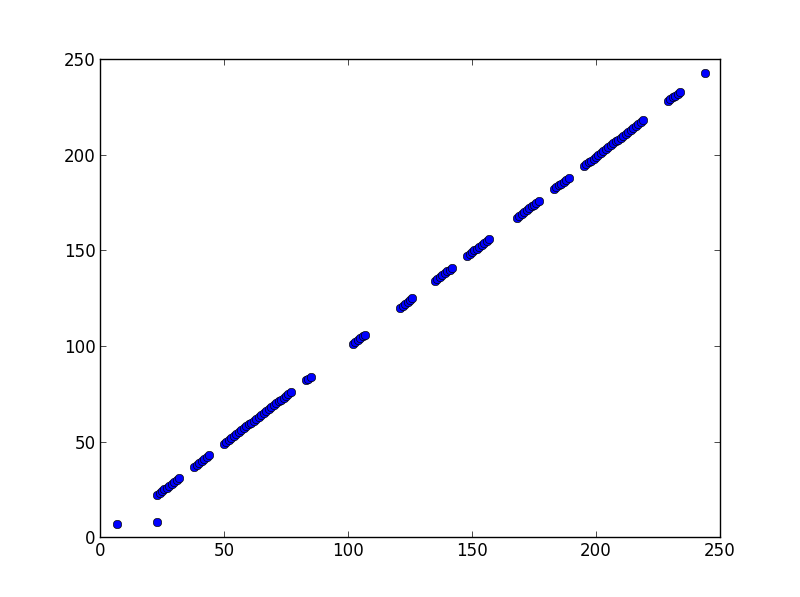
\includegraphics[width=0.6\linewidth]{../DogCatAlignment.png}
\captionof{figure}{Dog - cat alignment for the ELANE gene. 5 character region match.}
\end{center}

From the result of the alignment I eventually plotted a phylogenetic tree for the humaan, the chimpanzee, the dog and the cat:

\lstinputlisting[language=Python]{../PhylogeneticTree.py}

The figure below shows the output of the code above:

\begin{center}
\centering
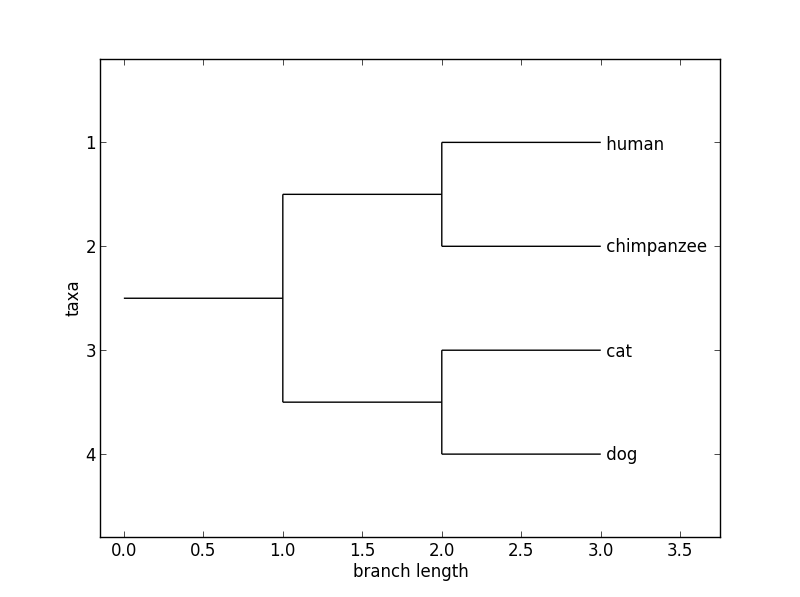
\includegraphics[width=0.6\linewidth]{../PhylogeneticTree.png}
\captionof{figure}{Phylogenetic tree for the humaan, the chimpanzee, the dog and the cat.}
\end{center}

%% Bibliographie unter Verwendung von dinnat %%%%%%%%%%%%%%%%%%%%%%%%%%
%\setbibpreamble{Präambel}		% Text vor dem Verzeichnis
%\bibliographystyle{dinat}
%\bibliography{bibliographie}	% Sie benötigen einen *.bib-Datei

\end{document}

